\documentclass[12pt]{article}

\usepackage{fullpage}
\usepackage[cm-default]{fontspec}
\usepackage{xgreek}
\usepackage{float}
\usepackage{xunicode}
\usepackage{xltxtra}
\usepackage{algorithm}
\usepackage{algpseudocode}
\usepackage{amsmath}
\usepackage{mathtools}
\usepackage{unicode-math}
\usepackage{fontspec}
\usepackage{caption}
\usepackage{subcaption}
\usepackage{soul}

\setmainfont{CMU Serif}

\title{Ανάπτυξη Λογισμικού για Πληροφοριακά Συστήματα}
\author{Πανγιώτης Φωτόπουλος\\
  \texttt{sdi1300195@di.uoa.gr}
  \and Μάνος Πιτσικάλης\\
  \texttt{sdi1300143@di.uoa.gr}}
\date{}

\begin{document}

\maketitle


\section{Βασικές Δομές - Γενικά}
Για την αποθήκευση του γράφου χρησιμοποιούνται δύο ευρετήρια (index-buffer) ένα για τις εξερχόμενες ακμές και ένα για τις εισερχόμενες ακμές. Στις αναζητήσεις και όπου χρείαζονται λίστες,για την αποφυγή πολλών malloc, χρησιμοποιούνται λίστες υλοποιημένες με πίνακα ,οι οποιές και επαναχρησιμοποιούνται όταν χρειάστει. Δηλάδη γινέται μια φορά malloc, αν χρειαστεί γίνεται realloc, και με την λήξη της εκτέλεσης γίνεται η αποδέσμευση της μνήμης. Επιπλέον στις αναζητήσεις και όπου αλλού χρειάζεται δομή αποθηκεύσης επίσκεψης π.χ.(στην bidirectional-bfs δομή visited) χρησιμοποιείται πίνακας A ίσος με των αριθμό των στοιχείων με versioning, δηλαδή αν το στοιχείο x έχει επισκεφτεί οταν γίνεται αναζήτηση με version v τότε A[x]=v, αν καποιό στοιχείο y δεν έχει επισκεφτεί τότε θα ισχύει A[y]<v ,έτσι η αρχικοποιήση γίνεται μόνο μία φορά καί ο έλεγχος γίνεται σε O(1).
\section{Λεπτομέρειες υλοποίησης Part 1}
\section{Λεπτομέρειες υλοποίησης Part 2}
\section{Λεπτομέρειες υλοποίησης Part 3}
\section{Δοκιμές στην υλοποίηση}
\section{Μετρήσεις}
Σύγκριση Part1 Part2 Part3\\
\begin{table}[H]
\caption{Dynamic Datasets times}

\begin{minipage}{.5\textwidth}
\footnotesize
\label{ddt}
\tabcolsep=0.11cm
\begin{tabular}{|l|l|l|l|}
\hline
\multicolumn{4}{|l|}{Dynamic Datasets times (MM:SS.000)} \\ \hline
          & Part 1      & Part 2     & Part 3-8 threads  \\ \hline
Tiny      & 00:00.001   & 00:00.002  & 00:00.004         \\ \hline
Small     & 00:00.453   & 00:00.519  & 00:00.596         \\ \hline
Medium    & 00:01.539   & 00:01.760  & 00:02.530         \\ \hline
Large     & 11:01.551   & 10:28.650  & 03:41.225         \\ \hline
Large 2   & 50:29.401   & 47:21.940  & 17:35.641         \\ \hline
\end{tabular}
\end{minipage}%
\begin{minipage}{.5\textwidth}
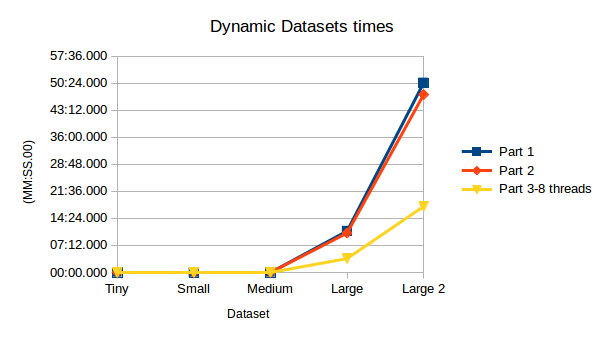
\includegraphics[scale=0.5]{DynamicDatasets_times.png}
\end{minipage}%
\end{table}

\begin{table}[H]
\caption{Dynamic Datasets Memory Usage}
\begin{minipage}{.5\textwidth}
\centering
\footnotesize
\tabcolsep=0.11cm
\label{ddm}
\begin{tabular}{|l|l|l|l|}
\hline
\multicolumn{4}{|l|}{Dynamic Dataset VmPeak (KB)} \\ \hline
         & Part 1 Vm & Part 2  & Part 3-8 threads \\ \hline
Large    & 1414896   & 1458116 & 2414616          \\ \hline
Large 2  & 1829748   & 2335964 & 3291848          \\ \hline
\end{tabular}
\end{minipage}%
\begin{minipage}{.5\textwidth}
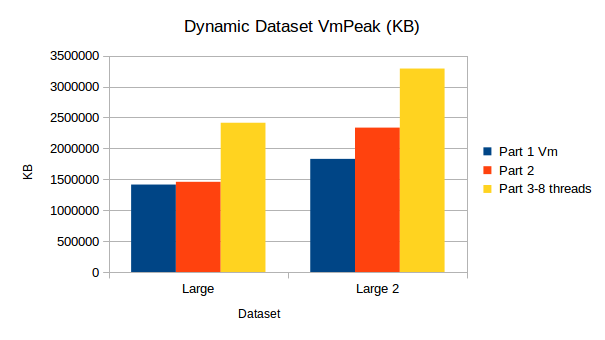
\includegraphics[scale=0.5]{DynamicDatasets_VmPeak.png}
\end{minipage}%
\end{table}

\begin{table}[H]
\caption{Static Datasets times}
\begin{minipage}{.5\textwidth}
\centering
\footnotesize
\tabcolsep=0.11cm
\label{sdt}
\begin{tabular}{|l|l|l|l|}
\hline
\multicolumn{4}{|l|}{Static Datasets times (MM:SS.000)} \\ \hline
        & Part 1         & Part 2    & Part 3-8 threads \\ \hline
Medium  & 00:01.434      & 00:02.538 & 00:02.637        \\ \hline
Large   & 05:03.604      & 01:54.640 & 00:51.800        \\ \hline
Large 2 & \textgreater3H & 26:28.035 & 08:31.369        \\ \hline
\end{tabular}
\end{minipage}%
\begin{minipage}{.5\textwidth}
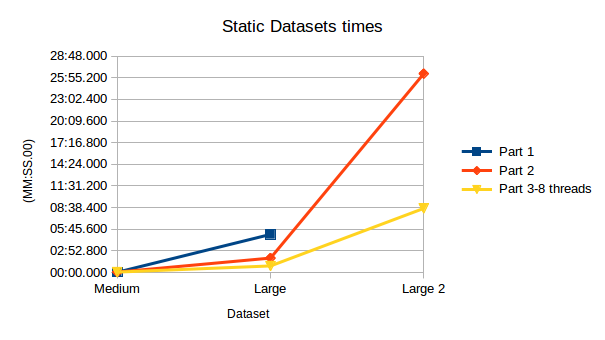
\includegraphics[scale=0.5]{StaticDatasets_times.png}
\end{minipage}%
\end{table}

\begin{table}[H]
\caption{Static Datasets Memory Usage}
\begin{minipage}{.5\textwidth}
\centering
\footnotesize
\tabcolsep=0.11cm
\label{sdm}
\begin{tabular}{|l|l|l|l|}
\hline
\multicolumn{4}{|l|}{Static Datasets times (MM:SS.000)} \\ \hline
        & Part 1         & Part 2    & Part 3-8 threads \\ \hline
Medium  & 00:01.434      & 00:02.538 & 00:02.637        \\ \hline
Large   & 05:03.604      & 01:54.640 & 00:51.800        \\ \hline
Large 2 & \textgreater3H & 26:28.035 & 08:31.369        \\ \hline
\end{tabular}
\end{minipage}%
\begin{minipage}{.5\textwidth}
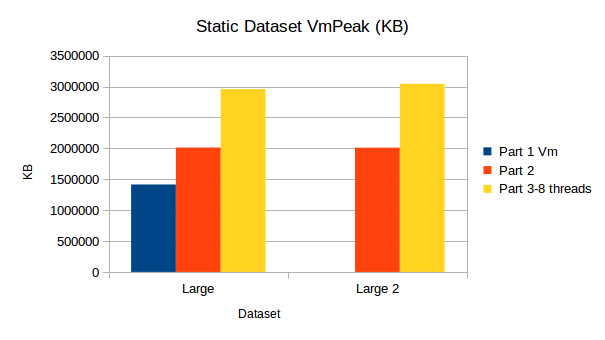
\includegraphics[scale=0.5]{StaticDatasets_VmPeak.png}
\end{minipage}%
\end{table}

Σύγκριση Part3 αριθμός νημάτων\\
\begin{table}[H]
\caption{Dynamic Dataset Multithreading times}
\begin{minipage}{.5\textwidth}
\centering
\footnotesize
\tabcolsep=0.11cm
\label{ddmt}
\scalebox{0.9}{
\begin{tabular}{|l|l|l|l|l|}
\hline
\multicolumn{5}{|l|}{Dynamic Dataset Multithreading times (MM:SS.000)} \\ \hline
Threads    & N=2          & N=4          & N=8          & N=16         \\ \hline
Large      & 05:57.266    & 04:03.300    & 03:41.225    & 03:42.664    \\ \hline
Large 2    & 26:30.534    & 18:45.376    & 17:35.641    & 17:57.566    \\ \hline
\end{tabular}}
\end{minipage}%
\begin{minipage}{.5\textwidth}
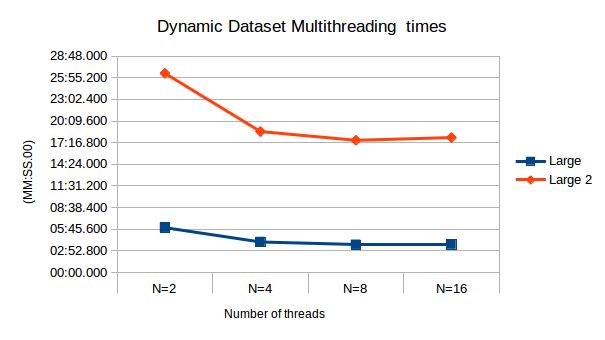
\includegraphics[scale=0.5]{DynamicDatasetMultithreading_times.png}
\end{minipage}%
\end{table}

\begin{table}[H]
\caption{Dynamic Dataset Multithreading Memory Usage}
\begin{minipage}{.5\textwidth}
\centering
\footnotesize
\tabcolsep=0.11cm
\label{ddmm}
\scalebox{0.9}{
\begin{tabular}{|l|l|l|l|l|}
\hline
\multicolumn{5}{|l|}{Dynamic Dataset Multithreading VmPeak(KB)} \\ \hline
Threads     & N=2        & N=4        & N=8        & N=16       \\ \hline
Large       & 1677284    & 1923060    & 2414616    & 3397252    \\ \hline
Large 2     & 2579536    & 2825312    & 3291848    & 4299972    \\ \hline
\end{tabular}
}
\end{minipage}%
\begin{minipage}{.5\textwidth}
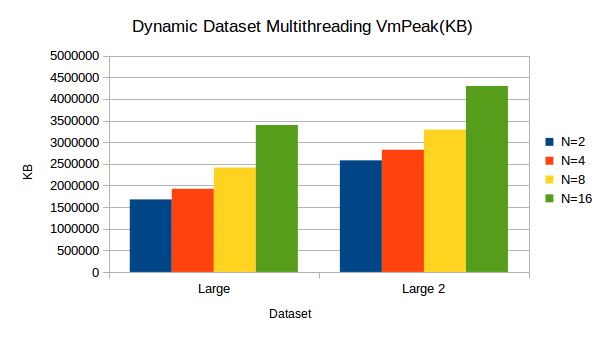
\includegraphics[scale=0.5]{DynamicDatasetMultithreading_VmPeak.png}\\
\end{minipage}%
\end{table}

\begin{table}[H]
\caption{Static Dataset Multithreading times}
\begin{minipage}{.5\textwidth}
\centering
\footnotesize
\tabcolsep=0.11cm
\label{sdmt}
\scalebox{0.9}{
\begin{tabular}{|l|l|l|l|l|}
\hline
\multicolumn{5}{|l|}{Static Dataset Multithreading times (MM:SS.000)} \\ \hline
Threads    & N=2          & N=4          & N=8          & N=16        \\ \hline
Large      & 01:53.454    & 01:18.555    & 01:01.018    & 00:51.800   \\ \hline
Large 2    & 16:54.585    & 10:05.976    & 08:30.127    & 08:31.690   \\ \hline
\end{tabular}
}
\end{minipage}%
\begin{minipage}{.5\textwidth}
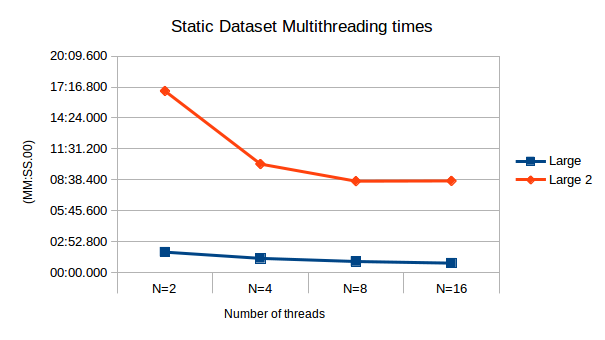
\includegraphics[scale=0.5]{DynamicStaticMultithreading_times.png}
\end{minipage}%
\end{table}

\begin{table}[H]
\caption{Static Dataset Multithreading Memory Usage}
\begin{minipage}{.5\textwidth}
\centering
\footnotesize
\tabcolsep=0.11cm
\label{sdmmu}
\scalebox{0.9}{
\begin{tabular}{|l|l|l|l|l|}
\hline
\multicolumn{5}{|l|}{Static Dataset Multithreading VmPeak(KB)} \\ \hline
Threads    & N=2        & N=4        & N=8        & N=16       \\ \hline
Large      & 2222564    & 2468340    & 2959892    & 3943000    \\ \hline
Large 2    & 2307580    & 2553356    & 3044908    & 3950336    \\ \hline
\end{tabular}
}
\end{minipage}%
\begin{minipage}{.5\textwidth}
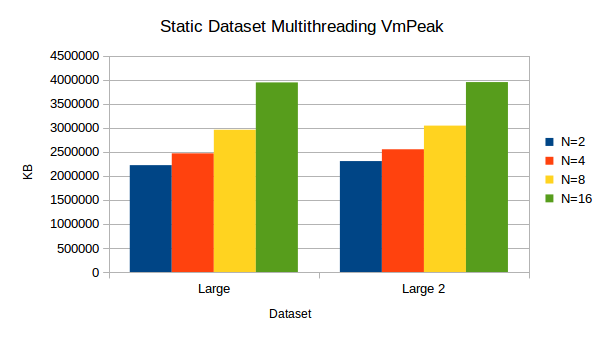
\includegraphics[scale=0.5]{DynamicStaticMultithreading_VmPeak.png}
\end{minipage}%
\end{table}
\end{document}
